%Template pembuatan proposal skripsi.
\documentclass{jtetiproposalskripsi}

%-----------------------------------------------------------------
%Disini awal masukan untuk data proposal skripsi
%-----------------------------------------------------------------
\titleind{KEAMANAN SISTEM TERDISTRIBUSI MENGGUNAKAN ALUR KONTROL INFORMASI}

\fullname{YUSUF WIBISONO}

\idnum{1110651202}

\approvaldate{11 Januari 2015}

\degree{Sarjana Teknik Informatika}

\yearsubmit{2015}

\program{Teknik Informatika}

\headprogram{Sarjiya, S.T., M.T., Ph.D.}

\dept{Teknik Informatika}

\firstsupervisor{Triawan, S.Kom, M.Kom}
%\firstnip{1976 0501 2002 12 1 002}

\secondsupervisor{Adi Cahyanto, S.Kom, M.Kom}
%\secondnip{1977 0131 2002 12 1 003}


%-----------------------------------------------------------------
%Disini akhir masukan untuk data proposal skripsi
%-----------------------------------------------------------------

\begin{document}

\cover

\approvalpage

%-----------------------------------------------------------------
%Disini akhir masukan untuk muka skripsi
%-----------------------------------------------------------------

%-----------------------------------------------------------------
%Disini awal masukan Intisari
%-----------------------------------------------------------------
\begin{abstractind}
Baru baru ini system operasi telah menunjukkan bahwa  \emph decentralized information flow control (DIFC) atau kontrol aliran informasi yang terdesentralisasi dapat mengamankan aplikasi yang dibangun dari kode yang mana sebagian besar tidak dapat mempercayainya. Disini kami memperluas pembahasan tentang DIFC ke jaringan. Kami menyajikan Dstar, sebuah sistem yang memberlakukan kebutuhan keamanan terhadap komponen yang saling dicurigai melalui kriptografi pada jaringan dan berfungsi sebagai mekanisme perlindungan local pada setiap OS hostnya. Dstar tidak memerlukan proses sepenuhnya akurat/terpercaya atau hardware, dan sangat berhati-hati  dalam membangun untuk menghindari rahasia pada saluran yang melekat dalam sebuah  \emph{interface}. Kami menggunakan Dstar untuk membangun server web bertingkat tiga yang meringankan efek dari aplikasi yang tidak dapat dipercaya dan kompromi terhadap \emph {hardware}.



\bigskip
\textbf{Kata kunci} :DIFC, Dstar, Kriptografi.
\end{abstractind}
%-----------------------------------------------------------------
%Disini akhir masukan Intisari
%-----------------------------------------------------------------

\tableofcontents
\addcontentsline{toc}{chapter}{DAFTAR ISI}
\selectlanguage{bahasa}\clearpage\pagenumbering{arabic}\setcounter{page}{1}

%-----------------------------------------------------------------
%Disini awal masukan untuk Bab
%-----------------------------------------------------------------
\chapter{LATAR BELAKANG}

\section{Latar Belakang Masalah}
Dewasa ini perkembangan system yang terkomputerisasi sangatlah pesat ditandai dengan adanya berbagai inovasi terhadap berbagai system yang pada intinya bertujuan untuk memudahkan para penggunanya dalam melakukan kegiatan kesehariannya. Berkaitan dengan adanya system yang terintegrasi sangatlah berkaitan erat dengan keamanan \emph{(security)} terhadap data ketika data tersebut berada dalam suatu jaringan, baik itu privasi data, keaslian data, dan lainnya. System terdistribusi mengatur mengenai masalah-masalah tersebut.



Dengan kata lain sistem ini melibatkan lebih dari satu komputer dalam suatu infrastruktur jaringan baik local,internet bahkan wireless. Sebuah sistem terdistribusi, tidak hanya melakukan komunikasi antara satu proses pada satu komputer dengan proses pada komputer yang lain, namun juga perlu mempertimbangkan ketersediaan infrastruktur jaringan yang memadai dan juga dukungan standarisasi sistem yang terbuka.

Sistem terdistribusi merupakan kebalikan dari Sistem Operasi Prosesor Jamak. Sistem terdisribusi mempunyai memori lokal pada setiap komponennya sehingga memungkinkan pembagian beban kerja, sedangkan Sistem operasi prosesor jamak menempatkan semua beban pekerjaan pada satu komponen saja.

Sistem terdistribusi memungkinkan penggunaan dan pengaksesan jarak jauh melalui jaringan TCP/IP, penggunaan resource pun dapat di minimalisir melalui sharing yang dilakukan pada jaringan seperi penggunaan printer pada jaringan lokal atau intranet.



\section{Tujuan Penelitian}
Membuat system keamanan pada system terdistribusi dengan menerapkan alur control informasi yang mana di dalamnya terdapat sebuah system yaitu Dstar.

\section{Manfaat Penelitian}




	

\vspace{-0.5cm}

\begin{enumerate}[a.]
\begin{singlespace}
\itemsep0em
\item Untuk mengetahui masalah pada system operasi.,
\item Untuk mengetahui kegiatan-kegiatan yang mencurigakan didalam sebuah system operasi.
\item Untuk pendeteksi dan pemberi peringatan terhadap 		gangguan yang datang dari luar dan dalam pada sebuah system.
\item Untuk pengamanan suatu system operasi.
\end{singlespace}
\end{enumerate}
	
	


%-------------------------------------------------------------------------------
\chapter{TINJAUAN PUSTAKA DAN DASAR TEORI}                

\section{Kriptografi}
Kriptografi (Cryptography) berasal dari bahasa yunani yaitu \emph{cryptos} artinya rahasia, sedangkan \emph{graphien} artinya tulisan, jadi kriptografi itu adalah tulisan rahasia. Dengan kata lain kriptografi adalah ilmu dan seni untuk menjaga kerahasiaan pesan dengan cara menyandikannya ke dalam bentuk yang tidak dapat dimengerti maknanya.
Dalam kriptografi ada beberapa istilah yang sering ditemukan yaitu \emph{“Plainteks}, dan \emph{Cipherteks”}. \emph{Plainteks} ada pesan atau teks jelas. Pesan bisa berisi data atau informasi yang dikirim oleh kurir, saluran telekomunikasi dan lain sebagainya. \emph{Cipherteks} adalah pesan yang tersandi. Kriptografi dibuat adalah untuk menghindari dari penyadap. Penyadap adalah orang yang mencoba melihat pesan saat dikirim.


\section{	DIFC \emph{(Desentralized Information Flow Control)}}
DIFC dapat mengamankan sebuah aplikasi yang telah di buat dari code yang mana sebagian besar sangat sulit untuk di percaya, dengan menggunakan mekanisme DIFC pun dapat mencegah dari adanya komunikasi yang mencurigakan dari komponen-komponen lainnya. Sementara itu DIFC sendiri merupakan sebuah OS \emph{(Operating System)} yang mana memungkinkan kita untuk mentolerir aplikasi-aplikasi yang akurat/terpercaya dan itu semua hanya dapat di lakukan hanya jika semua proses dijalankan pada \emph{hardware} yang sama. Pada umumnya DIFC digunakan pada sebuah situs web yang memiliki skala besar untuk banyak server, disisi lain untuk mencapai konfigurasi yang di inginkan ketika setiap komponen yang berjalan pada \emph{machine} yang terpisah juga dibutuhkan protocol jaringan yang mendukung DIFC. 


\section{HTTPS \emph{(Hypertext Transfer Protokol Secure)}}

\emph {Hypertext Transfer Protokol Secure} (HTTPS) adalah versi aman dari HTTP, protokol komunikasi dari \emph{World Wide Web}. Ditemukan oleh \emph{Netscape Communications Corporation} untuk menyediakan autentikasi dan komunikasi tersandi dan penggunaan dalam komersi elektris. HTTPS banyak digunakan protokol komunikasi untuk komunikasi yang aman melalui jaringan komputer, terutama dengan penyebaran luas di Internet. Secara teknis, itu bukan protokol itu sendiri, melainkan merupakan hasil dari hanya layering Hypertext Transfer Protocol (HTTP) di atas SSL / TLS protokol, sehingga menambah kemampuan keamanan dari SSL / TLS untuk standar komunikasi HTTP. Dalam banyak hal, https adalah identik dengan http, karena mengikuti protokol dasar yang sama. Klien http atau https, seperti Web browser, membuat sambungan ke server pada port standar. Ketika server menerima permintaan, ia mengembalikan status dan pesan, yang mungkin berisi informasi yang diminta atau menunjukkan kesalahan jika bagian dari proses berfungsi. Kedua sistem menggunakan Uniform Resource Identifier yang sama (URI) skema, sehingga sumber daya dapat universal diidentifikasi. Penggunaan https dalam skema URI bukan http menunjukkan bahwa sambungan terenkripsi yang diinginkan. Dalam penyebaran populer di internet, HTTPS menyediakan otentikasi dari situs web dan web server terkait yang satu berkomunikasi dengan, yang melindungi melawan Man-in-the-middle serangan. Selain itu, ia menyediakan enkripsi dua arah komunikasi antara klien dan server, yang melindungi terhadap penyadapan dan merusak dan / atau penempaan isi komunikasi. 

\section{SSL (Secure Sockets Layer)}
SSL adalah kependekan dari \emph{Secure Sockets Layer}, sebuah protokol yang dikembangkan oleh \emph{Netscape} untuk komunikasi dokumen yang membutuhkan privasi melalui Internet. SSL menggunakan suatu sistem enkripsi yang menggunakan dua kunci untuk melakukan enkripsi data. SSL adalah Protokol berlapis. Dalam tiap lapisannya, sebuah data terdiri dari panjang, deskripsi dan isi. SSL mengambil data untuk dikirimkan, dipecahkan kedalam blok-blok yang teratur, kemudian dikompres jika perlu, menerapkan MAC, dienkripsi, dan hasilnya dikirimkan. Di tempat tujuan, data didekripsi, verifikasi, dekompres, dan disusun kembali. Hasilnya dikirimkan ke klien di atasnya. 	

\section{RSA}
RSA di bidang kriptografi adalah sebuah algoritma pada enkripsi public key. RSA merupakan algoritma pertama yang cocok untuk digital \emph{signature} seperti halnya ekripsi, dan salah satu yang paling maju dalam bidang kriptografi \emph{public key}. RSA masih digunakan secara luas dalam \emph{protokol electronic commerce}, dan dipercaya dalam mengamankan dengan menggunakan kunci yang cukup panjang. 

\section{IDS \emph{(Intrusion Detection System)}}

Intrusion Detection System (disingkat IDS) adalah sebuah aplikasi perangkat lunak atau perangkat keras yang dapat mendeteksi aktivitas yang mencurigakan dalam sebuah sistem atau jaringan. IDS dapat melakukan inspeksi terhadap lalu lintas inbound  dan outbound dalam sebuah sistem atau jaringan, melakukan analisis dan mencari bukti dari percobaan intrusi (penyusupan).\\

Ada dua jenis IDS, yakni:
\vspace{-0.5cm}

\begin{enumerate}[a.]
\begin{singlespace}
\itemsep0em
\item Network based Intrusion Detection System (NIDS): Semua lalu lintas yang mengalir ke sebuah jaringan akan dianalisis untuk mencari apakah ada percobaan serangan atau penyusupan ke dalam sistem jaringan. NIDS umumnya terletak di dalam segmen jaringan penting di mana server berada atau terdapat pada "pintu masuk" jaringan. Kelemahan NIDS adalah bahwa NIDS agak rumit diimplementasikan dalam sebuah jaringan yang menggunakan switch Ethernet, meskipun beberapa vendor switch Ethernet sekarang telah menerapkan fungsi IDS di dalam switch buatannya untuk memonitor port atau koneksi. 
\item Host based Intrusion Detection System (HIDS): Aktivitas sebuah host jaringan individual akan dipantau apakah terjadi sebuah percobaan serangan atau penyusupan ke dalamnya atau tidak. HIDS seringnya diletakkan pada server-server kritis di jaringan, seperti halnya firewall, web server, atau server yang terkoneksi ke Internet.
 
\end{singlespace}
\end{enumerate}




\section{Dstar}
Dstar merupakan sebuah system yang memberlakukan keperluan keamanan terhadap komponen yang di curigai pada sebuah jaringan dan berfungsi sebagai mekanisme perlindungan pada setiap OS \emph{host}nya. Dstar tidak memerlukan waktu yang sepenuhnya akurat dan terpercaya dan sangat berhati-hati dalam membangun sebuah system yang bertujuan untuk menghindari rahasia yang terletak pada channel dalam sebuah \emph{interface}. Dstar digunakan untuk membangun sebuah server web tingkat tinggi dengan performa yang dapat meringankan efek dari aplikasi yang tidak akurat dan bersingkronisasi terhadap hardwarenya. Dstar dirancang untuk memenuhi tujuan sebagai berikut :
\vspace{-0.5cm}

\begin{enumerate}[a.]
\begin{singlespace}
\itemsep0em
\item Decentralized Trust \\ 
Ketika sebuah system operasi memilliki sebuah kemewahan dalam kernelnya yang sangat akurat terpercaya, sebuah system terdistribusi mungkin tidak memiliki kode yang sepenuhnya akurat untuk setiap hardware. Disini Dstar berusaha untuk memberikan hal yang  lebih umum, mekanisme desentralisasi yang memungkinkan aplikasi menggunakan otoritas seperti Verisign 1 oleh konvensi atau mengelola keakuratan mereka dengan cara lain.
\item Egalitarian mechanisms \\
Salah satu fitur kerja DIFC dari arus informasi sebelumnya sistem operasi kontrol adalah bahwa mekanisme DIFC adalah khusus dirancang untuk digunakan oleh aplikasi untuk setiap kodenya, tak peduli seberapa istimewanya kode tersebut DIFC masih dapat digunakan untuk melindungi data atau sejenis permission/izin lanjut. Property dalam komponen ini sangat memudahkan interaksi antar komponen yang saling berinteraksi antar komponen yang saling dicurigai keamanannya, ini merupakan salah satu kunci untuk menjaga keamanan dalam menghadapi keakuratan sebuah kode keamanan. 
\item No inherent covert channels \\
Tidak ada sistem kontrol aliran pada sebuah channels yang mengakibatkan  Informasi rahasia yang ada pasti akan memungkinkan beberapa komunikasi yang melanggar kebijakan throughcovert saluran. Namun bagaimanapun, sebuah aplikasi yang berbeda memiliki kepekaan yang berbeda pula untuk sebuah kode yang terlindungi dalam sebuah channel bandwith. Untuk memastikan bahwa Dstar dapat beradaptasi dengan kebutuhan keamanan yang berbeda , Tujuan kami adalah untuk menghindari saluran rahasia yang terdapat dalam antarmuka. Hal ini memungkinkan setiap saluran rahasia untuk dikurangi dalam penyebaran tertentu tanpa melanggar kompatibilitas. Menghindari saluran rahasia yang sangat rumit dengan keakuratan desentralisasi , bahkan tampaknya tindakan berbahaya seperti query server untuk otorisasi atau mengalokasikan memori untuk menyimpan sertifikat dapat secara tidak sengaja membocorkan informasi .
\item 
\end{singlespace}
\end{enumerate}


\section{\emph {Dstar Exporter}}
Faktanya  model untuk semua proses yang melakukan akses langsung ke sebuah jaringan tertentu dapat bertukar pesan, Dstar mengharuskan semua proses tersebut memiliki label yang sama contohnya Lnet  yang biasa di sebut dengan label the network (untuk jaringan yang terhubung ke internet). Hal ini di tujukan untuk memberikan batasan komunikasi terhadap kode yang berpotensi memiliki keakuratan data dan membutuhkan proses yang berjalan berbeda dengan label yang berbeda pula. Setiap host menjalankan daemon exporter yang merupakan satu-satunya proses yang mengirim dan menerima pesan langsung dari Dstar melalui jaringan. Ketika kedua proses pada mesin yang berbeda berkomunikasi melalui Dstar, mereka bertukar pesan-pesan melalui exporter local mereka, seperti yang di tunjukkan pada gambar berikut :




\begin{figure}[ht!]
  \centering
    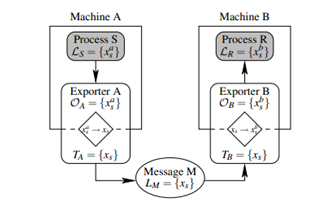
\includegraphics{gambar/dstar}
    \caption{Gambar 2.1. Proses jalannya Dstar Exporter}
    \label{iqrf}
\end{figure}

Gambar diatas menunjukkan bahwa pesan dikirim melalui proses S di machine A ke proses R di machine B L and O mendesign label OS lokal dan OS kepemilikan Xas dan Xbs adalah kategori OS kerahasiaan lokal . Eksportir menerjemahkan antara kategori OS dan Dstar global yang berarti kategori Xs.

\section{Antarmuka \emph{Exporter}}
Eksportir menyediakan pengiriman pesan satu arah yang belum bisa diandalkan ke arah titik akhir komunikasi yang disebut dengan slot, yang mana merupakan berupa pesan analog ke port pesan. Komunikasi ini belum bias di andalkan untuk menghindari potensi saluran yang bersifat rahasia melalui pesan tersebut, misalnya jika terdapat proses S dapat mengirim pesan ke R tetapi tidak sebaliknya, status pengiriman sms dapat mengizinkan R untuk menyampaikan informasi ke S dengan salah satunya menyetujui atau menolak pesan. Namun, pada umumnya dalam kasus dimana label memungkinkan komunikasi dua arah, kode yang terkumpul dibagian luar pada exporter menyediakan tingkat abstraksi yang lebih tinggi seperti RPC.banyak cara RPC untuk dapat menempatkan pada titik tertinggi yang mana arusnya belum bias dipercaya seperti UDP dan IP.

\section{Manajemen \emph{Service}}
Dstar eksportir menyediakan fungsionalitas tambahan untuk mengurusi dan bootstrapping, diimplementasikan sebagai RPC server yang dikenal dengan sebutan slot. Selanjutnya akan dijelaskan bagaimana mereka digunakan dalam sebuah aplikasi. Sebuah pelayanan delegasi mengizinkan sebuah proses yang memiliki kategori dalam system operasi local untuk mendelegasikan keakuratan dari kategori Dstar yang sesuai dengan exporter lain, yang di beri nama public key. Pemetaaan service membuat sebuah pemetaan antara Dstar kategori dan mekanisme keamanan system operasi local.

\section{\emph{Histar Exporter}}  
HiStar adalah sebuah sistem operasi baru yang dirancang untuk meminimalkan jumlah kode yang ada dalam sebuah sistem. HiStar menyediakan kontrol aliran informasi yang ketat, yang memungkinkan pengguna untuk menentukan kebijakan keamanan data yang tepat tanpa terlalu membatasi struktur aplikasi. Fitur keamanan HiStar dibuat agar memungkinkan untuk mengimplementasikan lingkungan Unix dengan kinerja yang dapat diterima hampir seluruhnya di perpustakaan user level yang akurat. Sistem ini tidak memiliki gagasan superuser, dan tidak ada kode sepenuhnya selain kernel. Fitur HiStar yang mengizinkan beberapa aplikasi baru, termasuk proses login dan pemisahan data antara jaringan pribadi virtual dan privasi.


\begin{figure}[ht!]
  \centering
    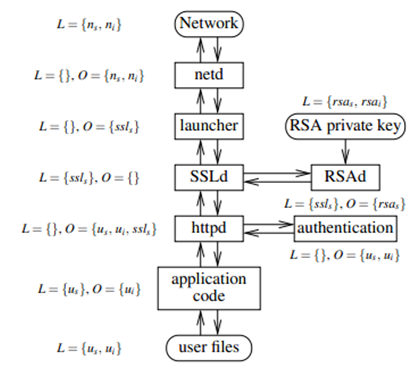
\includegraphics{gambar/histar}
    \caption{Gambar 2.2.Arsitektur dari Histar SSL web server, gambar kotak menyajikann tentang proses, dan gambar bulat menyajikan device dan file.}
    \label{star}
\end{figure}

\section{Web server Pada Histar}
Gambar diatas menunjukkan keseluruhan rancangan dari keistimewaan dari web server SSL. Web server dibangun dari sejumlah komponen yang saling dicurigai untuk mengurangi efek dari setiap komponen tunggal. TCP/IP menumpuk di Histar yang di implementasikan oleh user dan prosesnya di sebut dengan netd, yang memiliki akses langsung ke kernel devices. netd menyediakan socket interface ke aplikasi lain dalam sebuah system, yang digunakan oleh server web untuk mengakses jaringan. Koneksi pengguna yang pada awalnya ditangani oleh launcher yang menerima koneksi masukan dari browser dan memulai proses yang diperlukan untuk menanganinya.
\section{Keamanan Web Server} 
Pada Histar arsitektur web server yang tidak memiliki hirarki hak istimewa dan tidak ada komponen yang sepenuhnya yang dipercaya dan sebagai gantinya sebagian besar komponen yang saling curiga biasanya terbatas pada satu pengguna, yaitu penyerangnnya sendiri. Komponen terbesar dalam server web, SSLd dan kode aplikasi yang minimal dapat dipercaya dan tidak bias mengetahui data dari masing-masing pengguna bahkan jika mereka di deteksi berbahaya atau mencurigakan. Kode aplikasi di batasi oleh ategori kerahasiaan pengguna. Meskipun kode aplikasi memiliki kategori integritas pengguna namun kode ini hanya memberikan hak untuk menulis file kepada pengguna dan tidak untuk di explore ke pihak-pihak lain.

\section{\emph{Distributed web server}}

\begin{figure}[ht!]
  \centering
    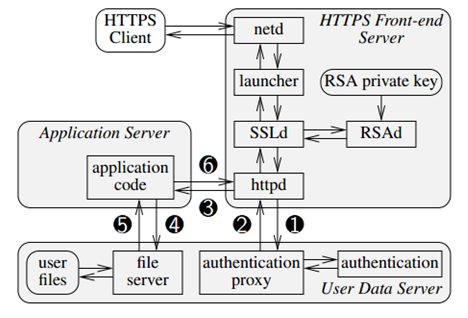
\includegraphics{gambar/web}
    \caption{Gambar 2.3. Struktur dari web server yang running pada multiple Histar hardware}
    \label{star}
\end{figure}

HTTPS front-end server menjalankan komponen yang bertanggung jawab untuk menerima klien koneksinya dan penanganan protokol HTTP Aplikasi server menjalankan kode application untuk mengeksekusi permintaan. Akhirnya, server data pengguna menyimpan data pengguna pribadi dan melakukan otentikasi pengguna. HTTPS dan server aplikasi sebagian besar state less sehingga mudah untuk meningkatkan kinerja secara keseluruhan dengan menambahkan mesin fisik lagi. Ini adalah pertimbangan penting untuk aplikasi web yang kompleks, di mana tugas-tugas sederhana seperti menghasilkan dokumen PDF dapat dengan mudah mengkonsumsi 100 milidetik waktu CPU (menggunakan GNU Ghostscript). Server data pengguna juga dapat dipartisi atas mesin multi-ple, dengan menjaga pemetaan konsisten dari tiap individu kepada pengguna data server tertentu secara bertanggung jawab untuk data mereka. Web server didistribusikan kami tidak memiliki otoritas pusat,dan semua server data saling curiga. Untuk web layanan yang menghasilkan bentuk pajak, ini memungkinkan beberapa perusahaan untuk masing-masing memberikan data server mereka sendiri. Sementara mungkin setiap perusahaan percaya layanan web untuk menghasilkan satu formulir pajak karyawan, tidak ada perusahaan mempercayai orang lain dari diri mereka sendiri dengan semua data karyawan mereka.Demikian pula, bagian yang berbeda dari data pengguna tunggal dapat ditangani oleh front-end dan server aplikasi yang berbeda.

\section{ \emph{Bootstrapping}}
Ketika menambahkan mesin baru untuk web yang kami distribusikan ke Server, mekanisme bootstrap diperlukan untuk memperoleh akses pada memori mesin baru dan sumber daya CPU. Untuk analogi, mempertimbangkan proses penambahan baru machine ke sebuah cluster Linux yang sudah ada Administrator
akan menginstal Linux, maka dari konsol mengatur root
password, mengkonfigurasi server ssh, dan  mencatat kunci ssh host untuk masuk pada hardware lainnya dan merupakan kemampuan untuk mengalokasikan dan deallocate semua memory dan proses yang digunakan oleh server web didistribusikan pada setiap mesin. Hal ini dapat dianggap sebagai "sumber daya alokasi tion root" untuk aplikasi tertentu.Namun, ada sudah tidak setara "root akses data." Sebaliknya, berbeda kategori-kategori melindungi bagian yang berbeda dari data.




%-------------------------------------------------------------------------------
\chapter{METODOLOGI}

\section{Studi literatur}


Pada tahap in, dilakukan pencarian informasi dan berbagai referensi mengenai topik yang dibahas dalam proposal, seperti tentang konsep dasar dari system terdistribusi, mekanisme keamanan dalam sebuah jaringan, berbagai system keamanan yang digunakan dalam sebuah keamanan jaringan yang nantinya akan dikaji dan dijadikan acuan dalam mengembangkan topik yang diajukan.
\section{Perancangan Desain Sistem}  
Pada tahap ini, di lakukan perancangan terhadap desain system yang akan dibuat dan nantinya digunakan pada DIFC itu sendiri. Contohnya seperti gambar dibawah ini :

\begin{figure}[ht!]
  \centering
    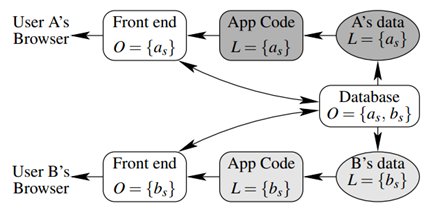
\includegraphics{gambar/metodologi}
    \caption{Gambar 3.1. contoh rancangan label}
    \label{star}
\end{figure}

Gambar diatas menunjukkan tentang contoh rancangan system penggunaan pada sebuah label untuk mencegah adanya kode aplikasi tentang ketidaktepatan data dengan menggunakan dua pengguna yaitu A dan B. Bulat, kotak merupakan proses, Ellips adalah pesan, sedangkan komponen yang berbayang di berikan label dengan kategori kerahasiaan pengguna, as dan bs untuk kategori masing-masing  A dan B. kemudian pada ujung bagian depan berkomunikasi dengan database untuk otentikasi pengguna dan mendapatkan hak kepemilikan dari kategori pengguna khusus.
Selanjutnya dilakukan perancangan terhadap web server pada Histar  SSL yang mana dibangun dari beberapa komponen yang bertujuan untuk mengantisipasi adanya kompromi dari single komponen yang lainnya. Pada implementasiannya TCP/IP  pada Histar diberikan pada pengguna yang prosesnya di sebut dengan netd, yang mana memiliki akses langsung ke kernel jaringan itu sendiri.

\begin{figure}[ht!]
  \centering
    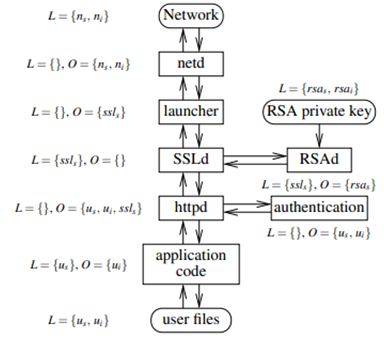
\includegraphics{gambar/arsitektur}
    \caption{Gambar 3.2. aritektur dari Histar SSL web server, gambar kotak menyajikann tentang proses, dan gambar bulat menyajikan device dan file.}
    \label{star}
\end{figure}

\section{Implementasi Sistem}
Pada tahap ini, ada beberapa hal yang perlu diperhatikan untuk memulai prosesnya diantaranya :
\subsection{manajemen sumber daya}
Web server yang didistribusikan juga harus secara eksplisit memberikan memori dan sumber daya CPU untuk semua pesan dan proses. Sejak launcher mendorong pelaksanaan pengguna permintaan, membutuhkan sumber daya tersebut pada semua mesin lainnya. untuk mengatur akses ke sumber daya tersebut, dan masing-masing aplikasi dan data server memiliki sebuah wadah awal berlabel  dan hanya di ketahui oleh launcher. . Peluncur memiliki ri, memberikan akses ke wadah awal pada mesin tersebut. Ketika peluncur mulai httpd terhadap kepemilikan ri, dan memberikan nama-nama ini wadah awal pada semua server lain. Ketika httpd berbicara dengan otentikasi proxy Langkah 1, misalnya, menggunakan wadah awal pada server data pengguna yang sesuai, bersama dengan kepemilikannya dari ri, untuk mengirim pesan permintaan. Karena HiStar member label pada  semua kontainer, server web harus berhati-hati untuk mengatur label yang sesuai ketika kode aplikasi ingin berkomunikasi dengan file server.
\subsection{Replikasi}
Setelah menambahkan mesin baru untuk cluster Dstar, yang administrator perlu aman meniru server web ke atasnya, dan khususnya, mentransfer kunci pribadi SSL untuk memulai proses RSAd baru. menggunakan replikasi khusus daemon untuk melakukan hal ini, yang menjamin bahwa kunci pribadi hanya mengungkapkan ke biner RSAd pada mesin remote Untuk mereplikasi RSAd, administrator menyediakan daemon ini dengan kunci publik dari mesin baru, dan akses ke sebuah wadah di atasnya (seperti dengan pemberian itu kepemilikan ri). Replikasi daemon menggunakan layanan pemetaan untuk membuat sebuah kategori baru rsans pada mesin baru, yang akan  melindungi kunci pribadi di sana. Untuk memastikan bahwa pribadi key tidak diteruskan ke proses yang salah, replikasi daemon menggunakan invocation untuk memohon Dijaga otentik Proses RSAd pada mesin baru dengan kepemilikan rsans , dan dibagikan kunci pribadi yang dilindungi dengan rsans.

\subsection{\emph{System Heterogen}}
Untuk menggambarkan bagaimana Dstar memfasilitasi penyebaran tambahan disini ditunjukkan bagaimana Linux dapat menggunakan HiStar atau Flume untuk mengeksekusi kode perl dipercaya dengan jaminan keamanan yang kuat dan juga diterapkan server Dstar RPC pada HiStar dan Flume yang mengambil source code dari script perl dan masukan data, mengeksekusi script pada masukan itu, dan mengembalikan perl s kode keluar dan output. Dstar menerjemahkan arus informasi pembatasan yang ditentukan oleh pemanggil ke HiStar atau Flume label, yang kemudian diberlakukan oleh sistem operasi. Layanan ini dapat digunakan oleh web Linux yang sudah ada server untuk aman mengeksekusi kode perl dipercaya. Linux Mesin dapat menentukan bagaimana berbagai contoh perl dapat berbagi data, dengan menentukan kebijakan menggunakan kerahasiaan dan integritas kategori dalam label permintaan itu. Untuk memastikan setiap permintaan diproses di isolasi lengkap, kerahasiaan segar dan kategori integritas dapat digunakan untuk setiap permintaan.
\subsection{Analisis Protokol}
Sumber utama ruang overhead dalam pesan Dstar adalah kunci public digunakan untuk nama kategori dan eksportir. Namun, kata kunci sering diulang beberapa kali dalam pesan yang sama. Sebagai contoh, pengguna kerahasiaan dan integritas kategori yang sering dibuat oleh eksportir yang sama, dan karena itu berbagi kunci publik yang sama. Selain itu, semua delegasi disertakan dalam pesan biasanya menyebutkan sama kunci publik eksportir pengiriman. Akibatnya, penekanan pesan hasil penghematan ruang yang signifikan, seperti ditampilkan dalam "kompresi". Namun, saat ini prototipe kami tidak menggunakan kompresi. Menyimpan hanya dari kunci publik dalam nama kategori dan dapat mengurangi ukuran, tetapi kemungkinan besar tidak akan mengurangi ukuran terkompresi.

\section{Analisis dan Uji Coba}
Untuk mengevaluasi kinerja aplikasi yang berjalan pada
Server web , kami mendekati layanan yang realistis kita beri beban kerja untuk generate ke PDF. Untuk setiap permintaan,HTTPS klien terhubung ke server dan perlengkapan usernam dan password. Web server menghasilkan 2 halaman Dokumen PDF berdasarkan pengguna file teks yang tersimpan 8KB di server, dan mengirimkannya kembali ke klien. . Siklus klien dimulai dengan melalui sejumlah kecil pengguna karena web
Server tidak terdeapat di setiap otentikasi, ini tidak
tidak condong kinerja. Dengan beberapa front-end server,
klien menggunakan kebijakan seleksi yang disebut dengan round-robin. Kami mengukur latency minimum yang diamati ketika klien tunggal adalah aktif, dan throughput maksimum dicapai dengan
jumlah optimal klien, sedangkan jumlah optimal klien umumnya sebanding dengan jumlah server. Sebuah web server dengan hak  istimewa dipisahkan berjalan pada HiStar menyediakan throughput 12 persen kurang dari Linux, perbedaannya adalah sebagian karena overhead dari garpu dan eksekusi pada HiStar. Pemisahan dari server web pada Menyebabkan Privilege HiStar mengakibatkan penalti 2 peren, dan pengguna layanan otentikasi HiStar itu,yang membutuhkan delapan panggilan gerbang, mengurangi throughput dengan lain 5 persen. Menjalankan server web didistribusikan pada sebuah hardware  menunjukkan overhead yang dikenakan oleh Dstar, meskipun begitu setup tidak akan digunakan dalam praktek Itu throughput beban kerja PDF memiliki skala baik dengan jumlah total server.
\begin{center}
Table 3.1. hasil uji coba kinerja aplikasi yang berjalan pada web server
\end{center}

\begin{figure}[ht!]
  \centering
    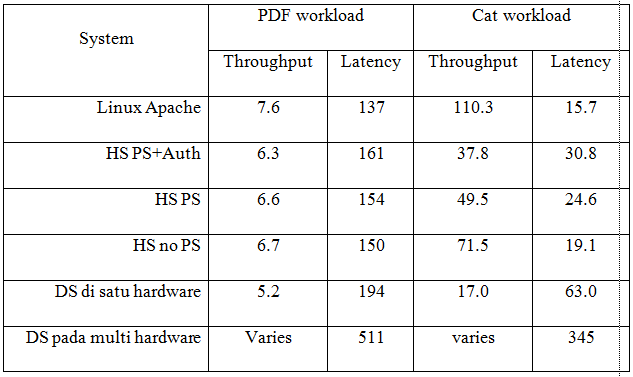
\includegraphics{gambar/tabel}
    \caption{}
    \label{star}
\end{figure}



%-----------------------------------------------------------------
%Disini akhir masukan Bab
%-----------------------------------------------------------------

%-----------------------------------------------------------------
%Disini awal masukan untuk Daftar Pustaka
%-----------------------------------------------------------------
%%\nocite{Abel2010,Guerbas201350}
%%\bibliography{research-plan}
%%\bibliographystyle{plainnat}
\begin{thebibliography}{9}

\bibitem[satu(2013)]{satu01}
O. Acıic¸mez, C¸ etin Kaya Koc¸, and J.-P. Seifert. On the power of simple branch prediction analysis. Cryptology ePrint Archive, Report 2006/351,2006.http://eprint.iacr.org/.


\bibitem[dua(2013)]{dua02}
J. P. Anderson. A unification of computer and network security concepts.In Proc. of the IEEE Symposium on Security and Privacy, pages 77–87,Oakland, CA, 1985.


\bibitem[tiga(2013)]{tiga03}
M. Blaze, J. Feigenbaum, and J. Lacy. Decentralized trust management. In Proc. of the IEEE Symposium on Security and Privacy, Oakland, CA, 1996.

\bibitem[empat(2013)]{empat04}
A. C. Bomberger, A. P. Frantz, W. S. Frantz, A. C. Hardy, N. Hardy, C. R.Landau, and J. S. Shapiro. The KeyKOS nanokernel architecture. InProc.of the USENIX Workshop on Micro-Kernels and Other Kernel Architec-tures,April 1992.


\bibitem[lima(2013)]{lima05}
D. Brumley and D. Boneh. Remote timing attacks are practical. InProc. of the 12th USENIX Security Symposium, August 2003.


\bibitem[enam(2013)]{enam06}
Dokumen online,https://openwrt.org/, diakses pada Maret 2013

\bibitem[tujuh(2013)]{tujuh07}
Dokumen online, http://www.digi.com/technology/rf-articles/wireless-zigbe,
diakses pada Maret 2013.
\bibitem[delapan(2013)]{delapan08}
M. Casado, T. Garfinkel, A. Akella, M. J. Freedman, D. Boneh, N. McKe own, and S. Shenker. SANE: A protection architecture for enterprise net-works. InProc. of the 15th USENIX Security Symposium, Vancouver, BC,
2006.
\bibitem[sembilan(2013)]{sembilan09}
T. Chothia, D. Duggan, and J. Vitek. Type-based distributed access control.
      In 16th IEEE Computer Security Foundations Workshop, pages 170–186.
      IEEE Computer Society, 2003.
\bibitem[sepuluh(2013)]{sepuluh10}
 D. E. Denning. A lattice model of secure information flow.Communica-tions    of the ACM, 19(5):236–243, May 1976.


\bibitem[sebelas(2013)]{sebelas11} D. Estrin. Non-discretionary controls for inter-organization networks. In
Proc. of the IEEE Symposium on Security and Privacy, pages 56–61, Oak-land, CA, 1985.
[10] H. Franke, R. Russell, and M. Kirkwood. Fuss, futexes and furwocks: Fast
userlevel locking in Linux. InProc. of the 2002 Ottawa Linux Symposium,
pages 479–495, June 2002.

\end{thebibliography}
\addcontentsline{toc}{chapter}{DAFTAR PUSTAKA}
%-----------------------------------------------------------------
%Disini akhir masukan Daftar Pustaka
%-----------------------------------------------------------------

\end{document}